\section{Problem Statement}
\label{sec:problem_statement}

\subsection{The Context and Naive Solution}

In real-world software development, object hierarchies are rarely static; they frequently evolve as new operational requirements emerge. To illustrate this, consider a typical graphics application managing a hierarchy of geometric elements, such as \texttt{Circle} and \texttt{Rectangle}, which both derive from a common \texttt{Shape} interface. 

Suppose a new business requirement dictates that the system must now serialize these elements to an external file. Under a conventional Object-Oriented paradigm—often deemed the naive solution—the intuitive approach is to embed a new pure virtual method, such as \texttt{save2File(std::string\& file)}, directly into the base \texttt{Shape} class. Consequently, this method must be overridden across all concrete derived classes. 

While this approach ostensibly leverages C++'s dynamic polymorphism, allowing the new operation direct access to the object's internal state, it tightly couples orthogonal behaviors (file I/O operations) with the core domain logic (geometric properties).

% PLACEHOLDER FOR CLASS DIAGRAM
\begin{figure}[H]
    \centering
    % Thay tên file ảnh của bạn vào đây
     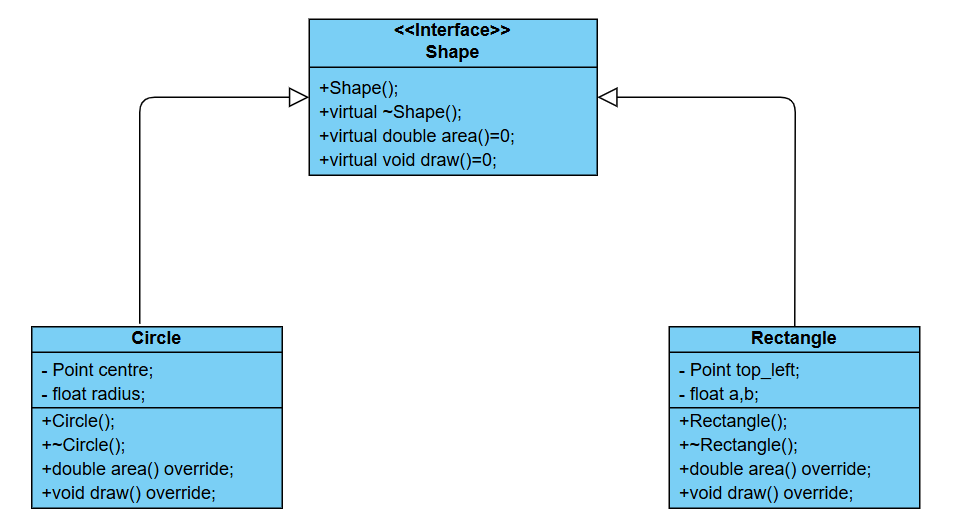
\includegraphics[width=0.7\textwidth]{Figures/assets/Naivesolution.png}
    \caption{Class Diagram illustrating the naive approach: embedding operations directly into the element hierarchy.}
    \label{fig:naive_diagram}
\end{figure}

The following C++ code snippet demonstrates this rigid structure, where adding a new feature requires modifying the base interface:

% PLACEHOLDER FOR C++ CODE
\begin{lstlisting}[language=C++, caption=Naive solution violating design principles.]
class Shape {
public:
    virtual ~Shape() = default;
    // Original Shape logic
    virtual void draw() = 0;
    virtual double area()=0;
    
    // NAIVE APPROACH: Adding a new operation directly modifies the base interface
    virtual void save2File(string& file) = 0; 
};

class Circle : public Shape {
private:
    Point centre;
    float radius;
public:
    void draw() override { /* ... */ }
    double area() override { /* ... */ }

    // new operator override
    void save2File(string& file) override { /* ... */ }
};

class Rectangle : public Shape {
private:
    Point top_left;
    float a,b;
public:
    void draw() override { /* ... */ }
    double area() override { /* ... */ }

    // new operator override
    void save2File(string& file) override { /* ... */ }
};
\end{lstlisting}

\subsection{Shortcomings of the Naive Solution}
While the naive approach appears straightforward initially, it introduces critical architectural and operational bottlenecks, particularly within C++ environments:

\begin{itemize}
    \item \textbf{Violation of the Single Responsibility Principle (SRP):} Forcing business logic classes to implement unrelated operations bloats the entities with orthogonal concerns. For instance, a shape class should not be burdened with the responsibility of saving data to external file.
    
    \item \textbf{Violation of the Open/Closed Principle (OCP):} Every time a new operation is introduced, the core base class and all its derived classes must be modified. The system is fundamentally ``open for modification,'' making the codebase brittle and prone to regression bugs \cite{gof1994}.
    
    \item \textbf{Recompilation Cascade and ABI Breakage:} This is a severe operational issue in C++. Modifying a base class header by adding new virtual functions alters the Virtual Method Table (\texttt{vtable}) layout, thereby breaking Application Binary Interface (ABI) compatibility. Consequently, every translation unit that includes the modified header must be recompiled, drastically increasing build times in large-scale projects \cite{iglberger2022}.
    
    \item \textbf{Restricted Source Code Accessibility:} In many practical scenarios, developers integrate third-party libraries, legacy codebases, or compiled SDKs. In such instances, modifying the original class structures is strictly prohibited or physically impossible due to a lack of source code access or organizational permissions.
\end{itemize}
